\chapter{Data exploration} % Main chapter title

\label{Chapter3} % For referencing the chapter elsewhere, use \ref{Chapter3} 

In this chapter, the approaches used in this research is examined. First, the join dataset merging from Last.fm and Spotify is mentioned. After that, the three algorithms and the evaluation metrics are discussed in detail.

\section{Dataset}

\subsection{Dataset creation}
The dataset for this thesis is a combination between two databases from two services: the 1K users dataset from Last.fm \footnote{https://last.fm} and the dataset crawling from Spotify Web Api \footnote{https://developer.spotify.com/web-api}. 

The dataset from Last.fm contains the listening habit from February, 2005 until May, 2009 for nearly 1000 users. The dataset contains more than 19 million entries, each entry consists of 4 attributes: the user id from Last.fm, the song that the user listened to, the artist who wrote the song, and the timestamp represents the time the user listened to the song. 

From the last.fm dataset, top 10000 songs that have the highest listening frequency are choosen. Then, track name and the respective artist are queried on Spotify API to get the corresponding track features. As Spotify API not only returns exact match but also similar match, and the name convention between the two systems might be different, a fuzzy matching algorithm is applied to filter the results. Particularly, the Levenshtein ratio is applied on the two fields. Any matching with a ratio higher than 80 percent is a good match, since the two strings are basically the same with some minor differences, which are the results of the different convention between the two system. Since matches with ratio between 60 and 80 percent might be good ones, manual check was done to guarantee the best result. I decided to cut off the result at 60 percent, as the majority of matches that are less than 60 percent are noisy and not accurate.

As some of the songs from Last.fm have yet been analyzed by Spotify, after joining the two datasets, the number of remaining songs is about 4200. I then remove users with less than 10 listening events.
The dataset is then divided into training set and test set following this rule: for each user, split the listening time into two halves, of which the first half belongs to the training set and the second half belongs to the test set. In the test set, all the tracks that are listened only 1 time are eliminated, as it is likely that the user only listened to it by chance. The final dataset contains with 891 users, 4200 unique tracks, and ...

\noindent The final dataset contains the following fields:

\begin{itemize}
\item[•] Username: The user who listen to the album, taken from last.fm database.
\item[•] Album: The name of the album the user listens to.
\item[•] Artist: The artist who performs the album.
\item[•] Playcount: The total number of time the user listens to the album.
\item[•] TrackId: The unique id of the track in Last.fm dataset, which also serves as unique key.
\item[•] Energy: A perceptual measurement of intensity and activity in a range from 0 to 1. The higher the score, the higher the energy the track contains. For example, metal rock has high energy, while a Bach prelude is perceived to have low energy. This measurement is built on top of dynamic range, loudness, timbral, onset rate, and general entropy.
\item[•] Speechiness: A measurement of how much spoken words is present compare to music. A value from 0.66 to 1 indicates that the track is mostly spoken words, such as talk show or audio book. Vice versa, a value between 0.33 and 0.66 implies that the track contains both music and speech, ranging from pop to rap music. A value below 0.33 indicates a non speech track. 
\item[•] Acousticness: A evaluation of how much acoustic a track contains compare to how much electronic. Again, a value closer to 1 implements that the track is played with mostly acoustic instruments, such as guitar and harmonica; while a value closer to 0 implements the present of electronic instruments.
\item[•] Danceability: A measurement of how suitable a track is for dancing based on a combination of musical elements including tempo, rhythm stability,  beat strength, and overall regularity. The higher the value, the more danceable the track.
\item[•] Tempo: The overall estimated tempo of a track, measuring in beats per minute (BPM).
\item[•] Instrumentalness: The assessment of how much a track incorporates vocals. The higher the instrumentalness, the greater likelihood the track contains no vocal content. 
\item[•] Key: The key (tonal center) a track is in. Integers map to pitches using Pitch Class notation \footnote{https://en.wikipedia.org/wiki/Pitch\_class}. 
\item[•] Valence: A measure from 0 to 1 of the positiveness of a track. Tracks with high valence sound more positive (e.g. happy, cheerful), and vice versa.
\item[•] Liveness: An indication of whether a track is performed live or in studio. The higher the liveness, the higher possibility that the track is performed live.
\item[•] Loudness: The overall loudness of a track in decibels (dB), with range from -60 to 0 db. 
\item[•] Mode: An indication of modality (major or minor) of a track. The field has only 2 values: 1 for major and 0 for minor.
\item[•] Time signature: An indication of how many beats are in each bar of a track. 
\end{itemize}

\subsection{Some descriptive data summarization}

In this section, some basic descriptive statistics of the data will be described, in order for the understanding of the overall picture of the data. Figure \ref{fig:boxplot} represent the boxplot diagrams of the energy, speechiness, acousticness, danceability, tempo, instrumentalness, valence, liveness, and loudness respectively. For key, mode, and time signature, as they are categorical variables, boxplot diagram information is not useful. Instead, for these variables, the frequency of the values, such as in table \ref{fig:freq_table} is displayed.

\begin{figure}
  \begin{subfigure}[b]{0.3\textwidth}
    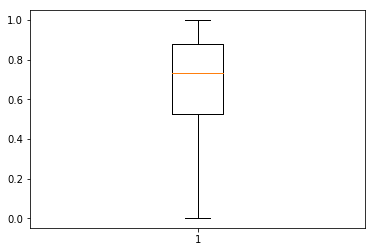
\includegraphics[width=\textwidth]{energy}
    \caption{Energy}
    \label{fig:energy}
  \end{subfigure}
  \hfill
  \begin{subfigure}[b]{0.3\textwidth}
    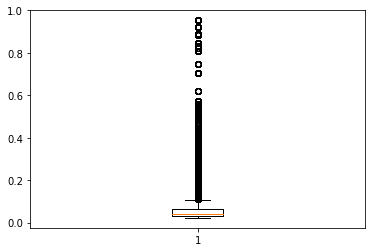
\includegraphics[width=\textwidth]{speechiness}
    \caption{Speechiness}
    \label{fig:speechiness}
  \end{subfigure}
  \hfill
  \begin{subfigure}[b]{0.3\textwidth}
    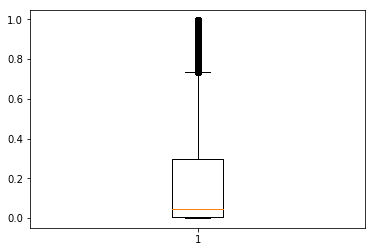
\includegraphics[width=\textwidth]{acousticness}
    \caption{Acousticness}
    \label{fig:acousticness}
  \end{subfigure}
  
  \bigskip
    \begin{subfigure}[b]{0.3\textwidth}
    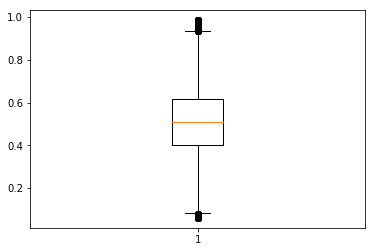
\includegraphics[width=\textwidth]{danceability}
    \caption{Danceability}
    \label{fig:danceability}
  \end{subfigure}
  \hfill
    \begin{subfigure}[b]{0.3\textwidth}
    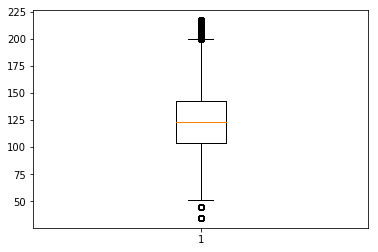
\includegraphics[width=\textwidth]{tempo}
    \caption{Tempo}
    \label{fig:tempo}
  \end{subfigure}
  \hfill
    \begin{subfigure}[b]{0.3\textwidth}
    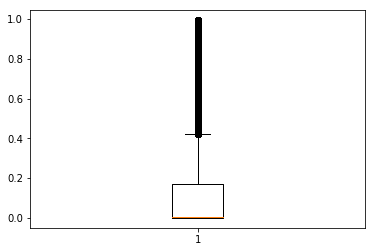
\includegraphics[width=\textwidth]{instrumentalness}
    \caption{Instrumentalness}
    \label{fig:instrumentalness}
  \end{subfigure}
  
  \bigskip
      \begin{subfigure}[b]{0.3\textwidth}
    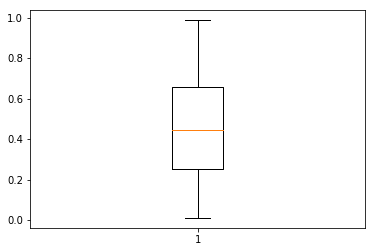
\includegraphics[width=\textwidth]{valence}
    \caption{Valence}
    \label{fig:valence}
  \end{subfigure}
  \hfill
    \begin{subfigure}[b]{0.3\textwidth}
    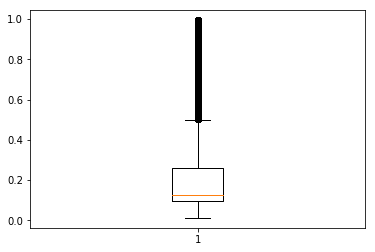
\includegraphics[width=\textwidth]{liveness}
    \caption{Liveness}
    \label{fig:liveness}
  \end{subfigure}
  \hfill
    \begin{subfigure}[b]{0.3\textwidth}
    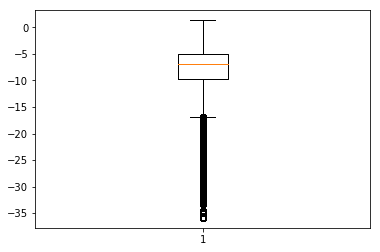
\includegraphics[width=\textwidth]{loudness}
    \caption{Loudness}
    \label{fig:loudness}
  \end{subfigure}
  
  \caption{Boxplot diagram of music features}
  \label{fig:boxplot}
\end{figure}

\begin{figure}
  \begin{subfigure}[b]{0.3\textwidth}
    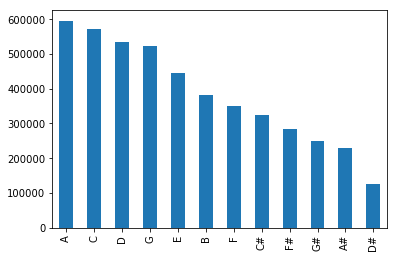
\includegraphics[width=\textwidth]{key}
    \caption{Key}
    \label{fig:key}
  \end{subfigure}
  \hfill
   \begin{subfigure}[b]{0.3\textwidth}
    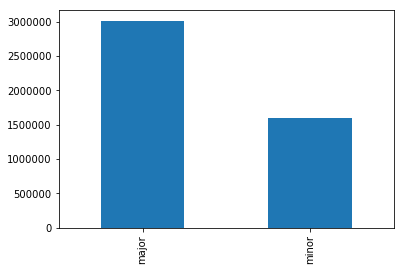
\includegraphics[width=\textwidth]{mode}
    \caption{Mode}
    \label{fig:mode}
  \end{subfigure}
  \hfill
  \begin{subfigure}[b]{0.3\textwidth}
    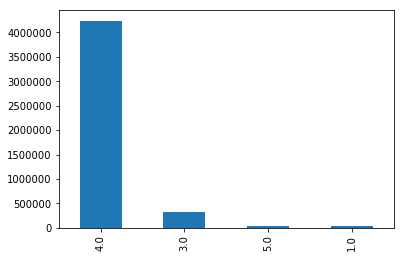
\includegraphics[width=\textwidth]{time_signature}
    \caption{Time signature}
    \label{fig:time_signature}
  \end{subfigure}
	
	\caption{Frequency table of music features}
	\label{fig:freq_table}
\end{figure}

\bigskip

\noindent We can see that from the diagrams:
\begin{itemize}
	\item Energy: the median is quite high, at nearly 0.8. However, the interquartile range of the energy is 0.35, suggesting that the energy spans equally across the value range.
	\item Speechiness: the median is at 0.04, with the first quartile at 0.03 and third quartile at 0.06, showing that most of the tracks have low level of spoken word. 
	\item Acousticness: the median is also at 0.04, with the first quartile at 0.003. However, the third quartile is at 0.3, suggesting that most of the tracks are not acoustic.
	\item Danceability: the median is at 0.5, with the first quartile at 0.4 and third quartile at 0.6, showing a normal distribution, which means that people listen equally to danceable track as well as undanceable track.
	\item Tempo: the median tempo is 123, with the first quartile of 104 and third quartile of 142, suggesting that most people listen to Allegro, which is fast and bright music.
	\item Instrumentalness: the median of 0.003 and the third quartile of 0.17 imply that most of the tracks contain vocal and not just pure instrument.
	\item Valence: with the median of 0.44, first quartile of 0.25, and third quartile of 0.66, valence also forms the normal distribution, suggesting that people listen equally to both positive and negative music.
	\item Liveness: the median of 0.12 and third quartile of 0.25 indicate that most tracks have a low level of liveness.
	\item Loudness: the first quartile of -9 and third quartile of -5 implement that most song have quite the same level of loudness.
	\item Key: songs with different key have different playing frequency. Overall, major key songs dominate minor ones.
	\item Mode: major key tracks are played more than minor ones, as previously stated.
	\item Time signature: the table indicates that more than 90\% of the tracks have 4 beats in each measure, around 7\% of the tracks have 3 beats in each measure, and the rest of the track have either 1 or 5 beats per measure.
\end{itemize}
	

